% Options for packages loaded elsewhere
\PassOptionsToPackage{unicode}{hyperref}
\PassOptionsToPackage{hyphens}{url}
\PassOptionsToPackage{dvipsnames,svgnames,x11names}{xcolor}
%
\documentclass[
  a4paper,
]{scrreport}

\usepackage{amsmath,amssymb}
\usepackage{lmodern}
\usepackage{iftex}
\ifPDFTeX
  \usepackage[T1]{fontenc}
  \usepackage[utf8]{inputenc}
  \usepackage{textcomp} % provide euro and other symbols
\else % if luatex or xetex
  \usepackage{unicode-math}
  \defaultfontfeatures{Scale=MatchLowercase}
  \defaultfontfeatures[\rmfamily]{Ligatures=TeX,Scale=1}
\fi
% Use upquote if available, for straight quotes in verbatim environments
\IfFileExists{upquote.sty}{\usepackage{upquote}}{}
\IfFileExists{microtype.sty}{% use microtype if available
  \usepackage[]{microtype}
  \UseMicrotypeSet[protrusion]{basicmath} % disable protrusion for tt fonts
}{}
\makeatletter
\@ifundefined{KOMAClassName}{% if non-KOMA class
  \IfFileExists{parskip.sty}{%
    \usepackage{parskip}
  }{% else
    \setlength{\parindent}{0pt}
    \setlength{\parskip}{6pt plus 2pt minus 1pt}}
}{% if KOMA class
  \KOMAoptions{parskip=half}}
\makeatother
\usepackage{xcolor}
\setlength{\emergencystretch}{3em} % prevent overfull lines
\setcounter{secnumdepth}{5}
% Make \paragraph and \subparagraph free-standing
\ifx\paragraph\undefined\else
  \let\oldparagraph\paragraph
  \renewcommand{\paragraph}[1]{\oldparagraph{#1}\mbox{}}
\fi
\ifx\subparagraph\undefined\else
  \let\oldsubparagraph\subparagraph
  \renewcommand{\subparagraph}[1]{\oldsubparagraph{#1}\mbox{}}
\fi


\providecommand{\tightlist}{%
  \setlength{\itemsep}{0pt}\setlength{\parskip}{0pt}}\usepackage{longtable,booktabs,array}
\usepackage{calc} % for calculating minipage widths
% Correct order of tables after \paragraph or \subparagraph
\usepackage{etoolbox}
\makeatletter
\patchcmd\longtable{\par}{\if@noskipsec\mbox{}\fi\par}{}{}
\makeatother
% Allow footnotes in longtable head/foot
\IfFileExists{footnotehyper.sty}{\usepackage{footnotehyper}}{\usepackage{footnote}}
\makesavenoteenv{longtable}
\usepackage{graphicx}
\makeatletter
\def\maxwidth{\ifdim\Gin@nat@width>\linewidth\linewidth\else\Gin@nat@width\fi}
\def\maxheight{\ifdim\Gin@nat@height>\textheight\textheight\else\Gin@nat@height\fi}
\makeatother
% Scale images if necessary, so that they will not overflow the page
% margins by default, and it is still possible to overwrite the defaults
% using explicit options in \includegraphics[width, height, ...]{}
\setkeys{Gin}{width=\maxwidth,height=\maxheight,keepaspectratio}
% Set default figure placement to htbp
\makeatletter
\def\fps@figure{htbp}
\makeatother

\usepackage{venndiagram}
\newcommand{\NN}{\mathbb{N}}
\newcommand{\ZZ}{\mathbb{Z}}
\newcommand{\QQ}{\mathbb{Q}}
\newcommand{\RR}{\mathbb{R}}
\newcommand{\CC}{\mathbb{C}}
\DeclareMathOperator{\operatorname{Int}}{Int}
\DeclareMathOperator{\operatorname{Ext}}{Ext}
\DeclareMathOperator{\operatorname{Fr}}{Fr}
\DeclareMathOperator{\Adh}{Adh}
\DeclareMathOperator{\Ac}{Ac}
\DeclareMathOperator{\sen}{sen}
\makeatletter
\makeatother
\makeatletter
\@ifpackageloaded{bookmark}{}{\usepackage{bookmark}}
\makeatother
\makeatletter
\@ifpackageloaded{caption}{}{\usepackage{caption}}
\AtBeginDocument{%
\ifdefined\contentsname
  \renewcommand*\contentsname{Tabla de contenidos}
\else
  \newcommand\contentsname{Tabla de contenidos}
\fi
\ifdefined\listfigurename
  \renewcommand*\listfigurename{Listado de Figuras}
\else
  \newcommand\listfigurename{Listado de Figuras}
\fi
\ifdefined\listtablename
  \renewcommand*\listtablename{Listado de Tablas}
\else
  \newcommand\listtablename{Listado de Tablas}
\fi
\ifdefined\figurename
  \renewcommand*\figurename{Figura}
\else
  \newcommand\figurename{Figura}
\fi
\ifdefined\tablename
  \renewcommand*\tablename{Tabla}
\else
  \newcommand\tablename{Tabla}
\fi
}
\@ifpackageloaded{float}{}{\usepackage{float}}
\floatstyle{ruled}
\@ifundefined{c@chapter}{\newfloat{codelisting}{h}{lop}}{\newfloat{codelisting}{h}{lop}[chapter]}
\floatname{codelisting}{Listado}
\newcommand*\listoflistings{\listof{codelisting}{Listado de Listados}}
\makeatother
\makeatletter
\@ifpackageloaded{caption}{}{\usepackage{caption}}
\@ifpackageloaded{subcaption}{}{\usepackage{subcaption}}
\makeatother
\makeatletter
\@ifpackageloaded{tcolorbox}{}{\usepackage[many]{tcolorbox}}
\makeatother
\makeatletter
\@ifundefined{shadecolor}{\definecolor{shadecolor}{rgb}{.97, .97, .97}}
\makeatother
\makeatletter
\makeatother
\ifLuaTeX
\usepackage[bidi=basic]{babel}
\else
\usepackage[bidi=default]{babel}
\fi
\babelprovide[main,import]{spanish}
% get rid of language-specific shorthands (see #6817):
\let\LanguageShortHands\languageshorthands
\def\languageshorthands#1{}
\ifLuaTeX
  \usepackage{selnolig}  % disable illegal ligatures
\fi
\IfFileExists{bookmark.sty}{\usepackage{bookmark}}{\usepackage{hyperref}}
\IfFileExists{xurl.sty}{\usepackage{xurl}}{} % add URL line breaks if available
\urlstyle{same} % disable monospaced font for URLs
\hypersetup{
  pdftitle={Talleres de Análisis Matemático},
  pdfauthor={Alfredo Sánchez Alberca},
  pdflang={es},
  colorlinks=true,
  linkcolor={blue},
  filecolor={Maroon},
  citecolor={Blue},
  urlcolor={Blue},
  pdfcreator={LaTeX via pandoc}}

\title{Talleres de Análisis Matemático}
\author{Alfredo Sánchez Alberca}
\date{6/1/22}

\begin{document}
\begin{titlepage}

%\AddToShipoutPicture*{\put(0,0){\includegraphics[scale=0.8]{img/background2}}} % Imagen de fondo, requiere el paquete eso-pic.
\begin{center}
\vspace*{5cm}

\Huge
{\textbf{\textsf{Talleres de Análisis Matemático}}}

\vspace{0.5cm}
\LARGE
{\textbf{\textsf{}}}

\vspace{1.5cm}


\includegraphics[width=0.4\textwidth]{img/logos/sticker.png}
\end{center}

\vfill

\begin{flushleft}
\begin{tabular}{ll}

\includegraphics[width=0.1\textwidth]{img/logos/aprendeconalf.png} & \parbox[b]{5cm}{\Large\textsf{Alfredo
Sánchez
Alberca}\\ \textsf{asalber@ceu.es} \\ \textsf{https://aprendeconalf.es}}
\end{tabular}
\end{flushleft}
\end{titlepage}\ifdefined\Shaded\renewenvironment{Shaded}{\begin{tcolorbox}[borderline west={3pt}{0pt}{shadecolor}, frame hidden, boxrule=0pt, enhanced, breakable, interior hidden, sharp corners]}{\end{tcolorbox}}\fi

\renewcommand*\contentsname{Tabla de contenidos}
{
\hypersetup{linkcolor=}
\setcounter{tocdepth}{2}
\tableofcontents
}
\bookmarksetup{startatroot}

\hypertarget{prefacio}{%
\chapter*{Prefacio}\label{prefacio}}
\addcontentsline{toc}{chapter}{Prefacio}

\markboth{Prefacio}{Prefacio}

Colección de talleres de Análisis Matemático aplicado.

\bookmarksetup{startatroot}

\hypertarget{anuxe1lisis-del-fractal-del-copo-de-nieve}{%
\chapter{Análisis del fractal del copo de
nieve}\label{anuxe1lisis-del-fractal-del-copo-de-nieve}}

El fractal del copo de nieve se construye partiendo de un triángulo
equilátero y alterando, de forma recursiva, cada segmento de línea de
las siguiente manera:

\begin{enumerate}
\def\labelenumi{\arabic{enumi}.}
\tightlist
\item
  Dividir el segmento de linea en tres partes iguales.
\item
  Dibujar hacia el exterior de la figura un triángulo equilátero a
  partir del segmento medio obtenido en el paso anterior.
\item
  Borrar el segmento medio obtenido en el primer paso.
\end{enumerate}

La siguiente figura ilustra el proceso para las 5 primeras iteraciones.

\begin{figure}

{\centering 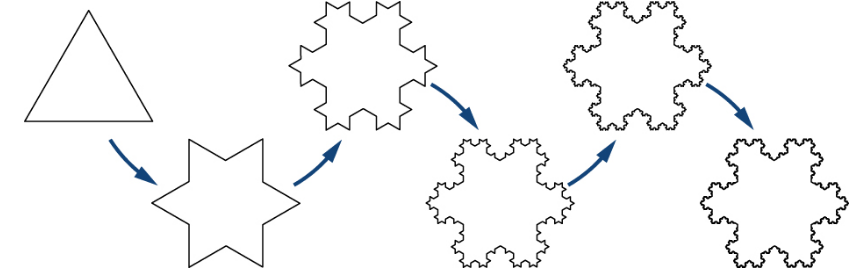
\includegraphics{./img/series/copo-nieve.png}

}

\caption{Creación del fractal del copo de nieve.}

\end{figure}

\begin{enumerate}
\def\labelenumi{\alph{enumi}.}
\tightlist
\item
  Estudiar la convergencia de la sucesión del número de lados.
\item
  Estudiar la convergencia de la sucesión de la longitud de los lados.
\item
  Estudiar la convergencia de la sucesión del perímetro del copo de
  nieve.
\item
  Calcular el area del copo de nieve en la etapa \(n\).
\item
  Calcular el area total del fractal del copo de nieve (cuando
  \(n\to \infty\)).
\end{enumerate}

\bookmarksetup{startatroot}

\hypertarget{sumas-de-riemann}{%
\chapter{Sumas de Riemann}\label{sumas-de-riemann}}

El cálculo de áreas encerradas por regiones del plano curvas ya fue
estudiado en la antigua Grecia. Una de las técnicas desarrolladas en
aquella época fue el
\href{https://es.wikipedia.org/wiki/M\%C3\%A9todo_por_agotamiento}{método
por agotamiento}, qué básicamente consistía en aproximar el área de la
región estudiada, inscribiendo en ella figuras geométricas de área
conocida.

En este taller trataremos de usar esta idea, usando \emph{sumas de
Riemann}, para aproximar el área que queda entre la gráfica de una
función \(f(x)=x^2\) y el eje \(X\), en el intervalo \(I=[0,1]\).

Para ello hay que seguir los siguientes pasos:

\begin{enumerate}
\def\labelenumi{\arabic{enumi}.}
\item
  Dar una aproximación por defecto y por exceso calculando las sumas
  inferior y superior de Riemann para particiones de \(I\) en \(n\)
  subintervalos de igual tamaño, para \(n=2, 5\) y \(10\).
\item
  Calcular la sumas inferior y superior de Riemann para particiones de
  \(I\) en \(n\) subintervalos de igual tamaño.
\item
  Calcular la integral inferior de Riemann mediante el límite cuando
  \(n\) tiende a \(\infty\) de la expresión obtenida en el apartado
  anterior para la suma inferior de Riemann.
\item
  Calcular la integral superior de Riemann mediante el límite cuando
  \(n\) tiende a \(\infty\) de la expresión obtenida en el apartado
  anterior para la suma superior de Riemann.
\item
  Calcular el área encerrada entre la gráfica de \(f\) y el eje \(X\) en
  el intervalo dado.
\item
  Generalizar el proceso anterior para calcular el área encerrada entre
  la gráfica de \(f\) y el eje \(X\) en un intervalo cualquiera
  \(I=[a,b]\).
\end{enumerate}

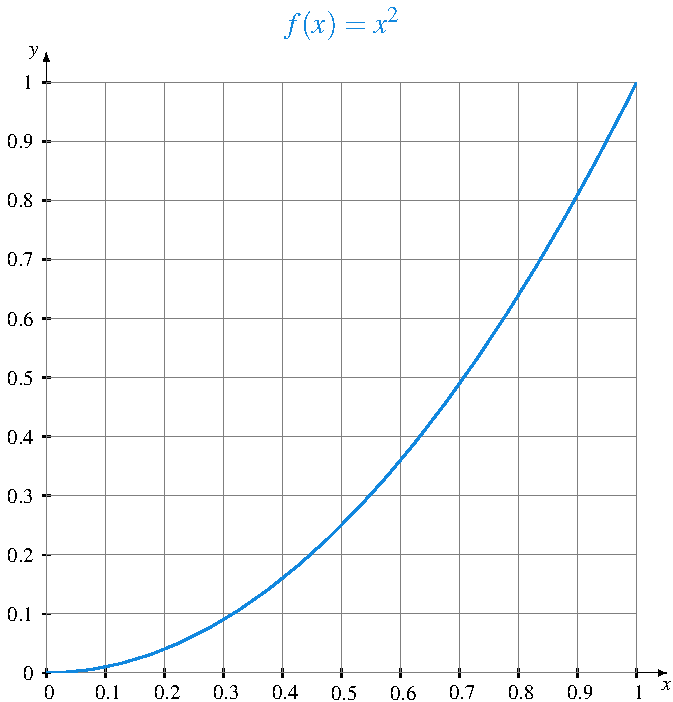
\includegraphics{./img/sumas-riemann/parabola-figure0.pdf}

\[
\sum_{i=1}^n i = \dfrac{n(n+1)}{2}\qquad \sum_{i=1}^n i^2 = \dfrac{n(n+1)(2n+1)}{6}
\]

\bookmarksetup{startatroot}

\hypertarget{teorema-fundamental-del-cuxe1lculo}{%
\chapter{Teorema Fundamental del
Cálculo}\label{teorema-fundamental-del-cuxe1lculo}}

El
\href{https://aprendeconalf.es/analisis-manual/09-integrales.html\#thm-teorema-fundamental-calculo-1}{Teorema
Fundamental del Cálculo} fue enunciado a la vez por Newton y Leibniz en
el siglo XVIII y establece el vínculo entre el Cálculo Diferencial y el
Cálculo Integral, que hasta entonces se habían desarrollado por caminos
muy diferentes.

En este taller trataremos de comprender esta conexión entre la derivada
y la integral estudiando cómo varía el área y volumen de algunas figuras
geométricas sencillas.

\begin{enumerate}
\def\labelenumi{\arabic{enumi}.}
\item
  Area de un cuadrado. ¿Cómo varía el área de un cuadrado si se
  incrementa el lado una cantidad infinitesimal \(dx\)? Dar una
  explicación geométrica. ¿Cómo se puede obtener el área de un cuadrado
  de lado \(a\) acumulando infinitas variaciones infinitesimales del
  area cada vez mayores?
\item
  Volumen de un cubo. ¿Cómo varía el volumen de un cubo si se incrementa
  el lado una cantidad infinitesimal \(dx\)? Dar una explicación
  geométrica. ¿Cómo se puede obtener el volumen de un cubo de lado \(a\)
  acumulando infinitas variaciones infinitesimales del volumen cada vez
  mayores?
\item
  Area de un círculo. ¿Cómo varía el area de un círculo si se incrementa
  el radio una cantidad infinitesimal \(dx\)? Dar una explicación
  geométrica. ¿Qué relación hay entre la fórmula del área y la del
  perímetro? ¿Cómo se puede calcular el área de un círculo de radio
  \(r\) acumulando infinitas variaciones infinitesimales del area cada
  vez mayores? ¿Qué otras formas se te ocurren de descomponer el área de
  un círculo para poder calcular su área mediante sumas de Riemann?
\item
  Volumen de una esfera. ¿Cómo varía el volumen de una esfera si se
  incrementa el radio una cantidad infinitesimal \(dx\)? Dar una
  explicación geométrica. ¿Qué relación hay entre la fórmula del volumen
  y la de la superficie? ¿Cómo se puede calcular el volumen de una
  esfera de radio \(r\) acumulando infinitas variaciones infinitesimales
  del volumen cada vez mayores? ¿Qué otras formas se te ocurren de
  descomponer el volumen de una esfera para poder calcular su área
  mediante sumas de Riemann?
\end{enumerate}

\bookmarksetup{startatroot}

\hypertarget{taller-de-anuxe1lisis-voluxfamenes-de-revoluciuxf3n}{%
\chapter{Taller de Análisis: Volúmenes de
revolución}\label{taller-de-anuxe1lisis-voluxfamenes-de-revoluciuxf3n}}

Los \emph{volúmenes} o \emph{sólidos de revolución} son figuras
geométricas en el espacio real que se obtienen rotando una función
\(y=f(x)\) alrededor del eje \(x\) o una función \(x=g(y)\) alrededor
del eje \(y\).

El volumen de estas figuras puede aproximarse mediante sumas de Riemann
de volúmenes de figuras geométricas regulares, típicamente cilindros o
anillos, y en última instancia puede calcularse mediante integrales
definidas.

En este taller se propone realizar el cálculo de los siguientes
volúmenes de revolución usando distintas estrategias para descomponer el
estas figuras en distintos tipos de figuras geométricas regulares.

\begin{enumerate}
\def\labelenumi{\alph{enumi}.}
\item
  \href{https://www.geogebra.org/m/nfdm8xjg}{Volumen de una esfera}
\item
  \href{https://www.geogebra.org/m/g2wu3tqw}{Volumen de una pirámide}
\item
  \href{https://www.geogebra.org/m/vfqyfuxx}{Volumen de un cono}
\item
  \href{https://www.geogebra.org/m/xugkcvn5}{Volumen de un paraboloide}
\item
  \href{https://www.geogebra.org/m/wy2uquqc}{Volumen de un toro}
\end{enumerate}



\end{document}
